% !TeX spellcheck = en_US

\chapter{Evaluation of the code generator}
\label{chap: code generator evaluation}
\section{Introduction}
By using model-driven engineering tools (MDE) tools for code generation, it is possible to generate software code automatically and achieve extremely high developer productivity rates of thousands of function points and millions of lines of code per person-month \cite{EvalCodeGen}. But, as we have seen in the previous chapters, the MDE approach consists of more than code generation tools; It defines the entire software-engineering approach that can impact the entire lifecycle from requirements gathering through sustainment \cite{CompBasedProcess, SAVOIR}.     

It is important to consider these tools and methods in the context of a particular system acquisition i.e., the MDE methods and tools need to be aligned with the system acquisition strategies, which would in turn improve system quality, reduce time to field, and reduce sustainment cost \cite{EvalCodeGen}. System acquisition strategies include: 

\begin{itemize}
\item Securing the necessary data rights and licensing for tools, models, generated code, run-time libraries, frameworks, and other supporting software
\item Reviewing and evaluating appropriate artifacts introduced by the MDE tools at the right time in the acquisition cycle
\item Approaches to manage program risks, include risk identification and mitigation 
\end{itemize}

If the methods and tools do not align with the system acquisition strategy, using them can result in increased risk and cost in development and sustainment\cite{EvalCodeGen}. The acquirers in government or large commercial enterprises have the challenge of selecting contractors to develop their systems. The tools and processes selected by the contractors and developers have direct impact on the software quality concerns of the acquirer, who often has little influence on the selection of these tools and processes. The tool acquirer would then have to answer the following acquisition evaluation questions \cite{EvalCodeGen}:

\begin{itemize}
\item Do the engineering processes and associated development tools match the desired acquisition strategy?
\item Do the tools support the developer's software development methodology?
\item Are the code generation tools capable of integrating with other development and management tools to support measurement and monitoring of the development progress?
\item Will the selected development methodology with its associated tools be available and compatible for the expected lifecycle of the system? 
\end{itemize}

This chapter subjects the code generator developed as a part of the Master thesis to evaluation methods listed in \cite{EvalCodeGen} and provide necessary inputs for conducting the acquisition evaluation.

\section{Selection and evaluation methods of a MDE tool for code generation}
The step-by-step MDE tool selection process defined in \cite{EvalCodeGen} makes use of the PECA method \cite{PECAProcess} as shown in \cref{fig: PECA method}.  

\begin{figure}[h]
	\centering
	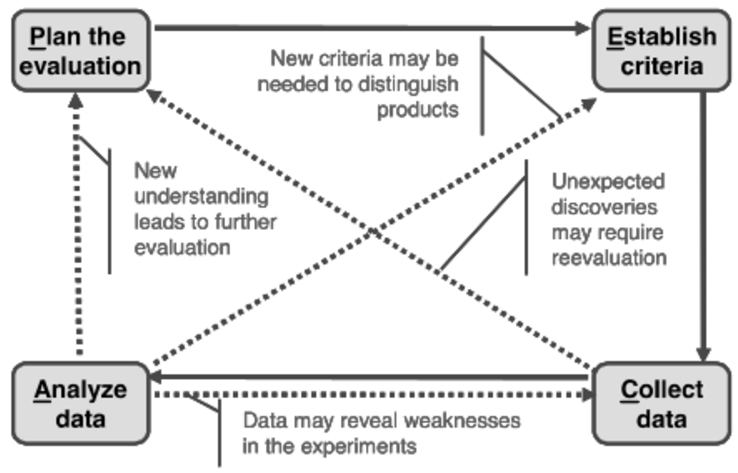
\includegraphics[width=0.5\textwidth]{PECAProcess.pdf}
	\caption{The PECA Process}
	\source{\cite{PECAProcess}}
	\label{fig: PECA method}
\end{figure}

As a part of the \texttt{Establish criteria} step in the PECA process, the acquirer must establish criteria with which he has to decide whether a particular tool for automatic code generation is suitable for a specific system acquisition. Such a criteria can be developed using risk taxonomy \cite{RiskTax} which ensures that all relevant acquisitions strategies are covered i.e., it provides a checklist to ensure all potential risks are considered \cite{EvalCodeGen}. The risk taxonomy has three main sections \cite{RiskTax}:

\begin{description}
\item [Product engineering] This covers activities that create a system that satisfies the specified requirements and customer expectations. Risks in this area generally arise from requirements that arise from requirements that are technically difficult to achieve, inadequate requirements and design analysis, or poor design and implementation quality 
\item [Development environment] This includes risks related to the development process and system, management methods, and work environment
\item [Program constraints] This cover risks that arise from factors external to the project 
\end{description}

To establish a criteria for a particular program/project, it is necessary for the program to first scan the risk taxonomy and identify those areas that apply for the project. Each risk creates one or more acquisition concerns , which may refine the program risk or indicate how certain tool features or capabilities might help mitigate the risk \cite{EvalCodeGen}.      

As part of the \texttt{Collect data} step in the PECA process, a vendor self-assessment questionnaire is prepared as in \cite{EvalCodeGen} which is given to the MDE tool vendors, to provide data needed to make the tool selection decision.

As a part of the \texttt{Analyze data} in the PECA rocess, it is then necessary to position these acquisition concerns in the specific program context and finally decide whether acquiring a particular tool is beneficial for the project.

In this Master thesis, a subset of evaluation criteria is chosen from Appendix A in \cite{EvalCodeGen}. The risk areas and the acquisition concerns which are meaningful in the scope of this Master thesis are chosen. Eg., the \cite{EvalCodeGen} discusses about potential risks in the Process Management area of the project and these are of no interest in this Master thesis and are not considered. Each of the acquisition concerns in Appendix A of \cite{EvalCodeGen} are then linked to the questions in the vendor self-assessment questionnaire listed in Appendix B of the \cite{EvalCodeGen}. For our chosen subset of potential areas and the acquisition concerns within this Master thesis, an attempt is made to answer the corresponding linked questions in the questionnaire.

% Please add the following required packages to your document preamble:
% \usepackage{multirow}
% \usepackage{graphicx}
\begin{table}[]
	\centering
	\caption{Evaluation Criteria - Product Engineering Risk Area (Requirements)}
	\label{my-label}
	\resizebox{\textwidth}{!}{%
		\begin{tabular}{lll}
			\hline
			\multicolumn{1}{|c|}{\textbf{Risk area}} & \multicolumn{1}{c|}{\textbf{\begin{tabular}[c]{@{}c@{}}Potential Acquisition \\ Concerns \\ Related to MDE Tools for \\ Automatic Code Generation\end{tabular}}} & \multicolumn{1}{c|}{\textbf{\begin{tabular}[c]{@{}c@{}}Answers to the linked questions \\ in the questionnaire\end{tabular}}} \\ \hline
			\multicolumn{3}{|l|}{\textbf{Requirements}} \\ \hline
			\multicolumn{1}{|l|}{\multirow{3}{*}{Stability}} & \multicolumn{1}{l|}{\begin{tabular}[c]{@{}l@{}}Responding to requirements \\ changes may necessitate \\ operating on partially complete \\ models and performing \\ refactoring or rework on \\ models.\end{tabular}} & \multicolumn{1}{l|}{\begin{tabular}[c]{@{}l@{}}The OBSW models designed using the OSRA Component \\ Model should be subjected to model validation against the \\ OSRA Specification Compliance and the SCM Metamodel \\ Compliance before it is subjected to automatic code \\ generation. In that case, the OBSW model, even if partially \\ complete can be subjected to code generation if it clears the \\ model validation step\end{tabular}} \\ \cline{2-3} 
			\multicolumn{1}{|l|}{} & \multicolumn{1}{l|}{\begin{tabular}[c]{@{}l@{}}Communication with stake-\\ holders is partially important \\ to resolve requirements issues, \\ so tool features that support \\ this become more important\end{tabular}} & \multicolumn{1}{l|}{\begin{tabular}[c]{@{}l@{}}It is possible to annotate each of the model entities while \\ constructing the OBSW model with information which \\ can be used for communicating with the stakeholders. \\ There is no additional documentation too which comes with \\ the OSRA SCM tool suite\end{tabular}} \\ \cline{2-3} 
			\multicolumn{1}{|l|}{} & \multicolumn{1}{l|}{\begin{tabular}[c]{@{}l@{}}Interfaces between the soft-\\ ware modeling tools and \\ the requirements management \\ tools promote co-evolution \\ of requirements and software\end{tabular}} & \multicolumn{1}{l|}{\begin{tabular}[c]{@{}l@{}}There is no support for tracing requirements into model \\ elements at the current state of development of OSRA\\ SCM\end{tabular}} \\ \hline
			\multicolumn{1}{|l|}{\begin{tabular}[c]{@{}l@{}}Completeness\\ Clarity\\ Validity\end{tabular}} & \multicolumn{1}{l|}{\begin{tabular}[c]{@{}l@{}}In addition to the concerns \\ noted above about require-\\ ments stability, the ability to \\ execute or simulate the exe-\\ cution of the model can help\\ validate requirements \\ completeness\end{tabular}} & \multicolumn{1}{l|}{\begin{tabular}[c]{@{}l@{}}At the current stage of the development of the OSRA \\ SCM, it is not possible visualize the execution of the model. \\ It is only possible to create static models of the OBSW \\ and it is not possible to trace the flow of execution \\ through the model, or inject data or events into the model\end{tabular}} \\ \hline
			\multicolumn{1}{|l|}{Feasibility} & \multicolumn{1}{l|}{\begin{tabular}[c]{@{}l@{}}The ability to perform analysis \\ of the model for qualities \\ such as latency, throughput \\ and consistency can help \\ demonstrate the feasibility \\ of requirements\end{tabular}} & \multicolumn{1}{l|}{\begin{tabular}[c]{@{}l@{}}The model-based static analysis of the OBSW model is not \\ possible at the current stage of development of the OSRA. \\ Step 10 of the overall software development process \\ in \cref{section: Design steps} in chapter \cref{chap: Software development process} gives an idea about the \\ analysis of latency, throughput etc. which can be perform-\\ ed on the OBSW model in the future\end{tabular}} \\ \hline
			\multicolumn{1}{|l|}{Scale} & \multicolumn{1}{l|}{\begin{tabular}[c]{@{}l@{}}Limitation on the size or \\ complexity of the model \\ that can be represented,\\ analyzed, or transformed \\ by the tool will limit the scale \\ of the system that can be \\ created\end{tabular}} & \multicolumn{1}{l|}{\begin{tabular}[c]{@{}l@{}}There are no size and complexity limitations for representing \\ the OBSW models using the OSRA SCM tools\end{tabular}} \\ \hline
		\end{tabular}%
	}
\end{table}


% Please add the following required packages to your document preamble:
% \usepackage{graphicx}
\begin{table}[]
	\centering
	\caption{Evaluation Criteria - Product Engineering Risk Area (Design)}
	\label{my-label}
	\resizebox{\textwidth}{!}{%
		\begin{tabular}{lll}
			\hline
			\multicolumn{1}{|c|}{\textbf{Risk area}} & \multicolumn{1}{c|}{\textbf{\begin{tabular}[c]{@{}c@{}}Potential Acquisition \\ Concerns \\ Related to MDE Tools for \\ Automatic Code Generation\end{tabular}}} & \multicolumn{1}{c|}{\textbf{\begin{tabular}[c]{@{}c@{}}Answers to the linked questions \\ in the questionnaire\end{tabular}}} \\ \hline
			\multicolumn{3}{|l|}{\textbf{Design}} \\ \hline
			\multicolumn{1}{|l|}{Interfaces} & \multicolumn{1}{l|}{\begin{tabular}[c]{@{}l@{}}If only parts of the system \\ will be automatically gene-\\ rated, while other parts will \\ be developed using traditional \\ approaches, the interfaces bet-\\ ween these two types of \\ software must be designed \\ and developed\end{tabular}} & \multicolumn{1}{l|}{\begin{tabular}[c]{@{}l@{}}In the software design for the generated infrastructure code, \\ the model entities are mapped to infrastructural code\\ entities. As the model entities clearly separates the two \\ types of code, the generated infrastructural code entities\\ as well clearly separates the generated code from the user \\ code, which may be developed using traditional approaches. \\ The generated source code needs to be compiled. The \\ generated source code is in C++ and works with the \\ Tasking framework written in C++. The  code is generated\\ for the Linux platform and GCC C++-11 compiler can be \\ used to compile to the source code. The code generator\\ also generates SCons build scripts for building the generated\\ software code automatically\end{tabular}} \\ \hline
			\multicolumn{1}{|l|}{Testability} & \multicolumn{1}{l|}{\begin{tabular}[c]{@{}l@{}}The tool should generate code\\ that exposes internal states and \\ interfaces needed to test the\\ generated software\end{tabular}} & \multicolumn{1}{l|}{\begin{tabular}[c]{@{}l@{}}The generated infrastructural code is testable as testability\\ of the generated code is one of the main concerns in the\\ software design for the infrastructural code. (Effective test-\\ ability of the generated code is proven with an example in\\ the subsequent chapter)\\ Mock C++ classes for different infrastructural code entities\\ and automatic test cases can also be generated in future\\ using the code generator\end{tabular}} \\ \hline
			\multicolumn{1}{|l|}{\begin{tabular}[c]{@{}l@{}}Hardware\\ constraints\end{tabular}} & \multicolumn{1}{l|}{\begin{tabular}[c]{@{}l@{}}The generated code must be \\ sufficiently efficient (in terms of\\ processors, memory, network,\\ disk, and other resource utiliz-\\ ation) to operate in the target\\ environment\end{tabular}} & \multicolumn{1}{l|}{\begin{tabular}[c]{@{}l@{}}The generated code depends on Tasking framework written\\ in C++. Hence effective resource utilization eg., processor,\\ memory, network disk utilization is not of concern in this\\ Master thesis\end{tabular}} \\ \hline
			\multicolumn{1}{|l|}{\begin{tabular}[c]{@{}l@{}}Non-deve-\\ lopmental\\ software\end{tabular}} & \multicolumn{1}{l|}{\begin{tabular}[c]{@{}l@{}}Any runtime packages, librar-\\ ies, or other software required\\ to execute the generated code\\ must be known, compatible\\ with the current and future\\ target environments, and able\\ to be certified for use in other\\ environments\end{tabular}} & \multicolumn{1}{l|}{\begin{tabular}[c]{@{}l@{}}The generated code depends on Tasking framework which\\ is written in C++. The generated code uses Linux as the \\ target environment and hence uses Tasking framework\\ which sits on top of Linux POSIX library. As Tasking \\ framework is internal to DLR, no certification efforts have \\ been done. The compatibility of Tasking framework for \\ future environments is not of concern in this Master thesis.\\ The build system which is automatically generated by the\\ code generator makes use of SCons for building the\\ generated code\end{tabular}} \\ \hline
		\end{tabular}%
	}
\end{table}


% Please add the following required packages to your document preamble:
% \usepackage{graphicx}
\begin{table}[]
	\centering
	\caption{Evaluation Criteria - Product Engineering Risk Area (Integration and Test)}
	\label{my-label}
	\resizebox{\textwidth}{!}{%
		\begin{tabular}{lll}
			\hline
			\multicolumn{1}{|c|}{\textbf{Risk area}} & \multicolumn{1}{c|}{\textbf{\begin{tabular}[c]{@{}c@{}}Potential Acquisition \\ Concerns \\ Related to MDE Tools for \\ Automatic Code Generation\end{tabular}}} & \multicolumn{1}{c|}{\textbf{\begin{tabular}[c]{@{}c@{}}Answers to the linked questions \\ in the questionnaire\end{tabular}}} \\ \hline
			\multicolumn{3}{|l|}{\textbf{Integration and Test}} \\ \hline
			\multicolumn{1}{|l|}{Environment} & \multicolumn{1}{l|}{\begin{tabular}[c]{@{}l@{}}The generated code may have\\ run-time dependencies on third\\ party software or software \\ provided by the tool vendor.\\ This software must be compa-\\ tible with the integration\\ environment\end{tabular}} & \multicolumn{1}{l|}{\begin{tabular}[c]{@{}l@{}}The generated code has run-time dependencies on the \\ Tasking framework which is internal to DLR and no \\ integration tests are automatically generated at the moment \\ from the code generator\\ SCons build scripts are also automatically generated by the\\ code generator which helps in building the generated code\end{tabular}} \\ \hline
			\multicolumn{1}{|l|}{\begin{tabular}[c]{@{}l@{}}Product\\ System\end{tabular}} & \multicolumn{1}{l|}{\begin{tabular}[c]{@{}l@{}}The tool should generate code\\ that exposes internal states and\\ interfaces needed to test the \\ generated software code\end{tabular}} & \multicolumn{1}{l|}{\begin{tabular}[c]{@{}l@{}}The generated infrastructural code is testable as testability\\ of the generated code is one of the main concerns in the\\ software design for the infrastructural code. (Effective test\\ -ability of the generated code is proven with an example in\\ the subsequent chapter)\\ Mock C++ classes for different infrastructural code entities\\ and automatic test cases can also be generated in future\\ using the code generator\end{tabular}} \\ \hline
		\end{tabular}%
	}
\end{table}

% Please add the following required packages to your document preamble:
% \usepackage{graphicx}
\begin{table}[]
	\centering
	\caption{Evaluation Criteria - Program Constraints Risk Area (Resources)}
	\label{my-label}
	\resizebox{\textwidth}{!}{%
		\begin{tabular}{lll}
			\hline
			\multicolumn{1}{|c|}{\textbf{Risk area}} & \multicolumn{1}{c|}{\textbf{\begin{tabular}[c]{@{}c@{}}Potential Acquisition \\ Concerns \\ Related to MDE Tools for \\ Automatic Code Generation\end{tabular}}} & \multicolumn{1}{c|}{\textbf{\begin{tabular}[c]{@{}c@{}}Answers to the linked questions \\ in the questionnaire\end{tabular}}} \\ \hline
			\multicolumn{3}{|l|}{\textbf{Resources}} \\ \hline
			\multicolumn{1}{|l|}{Schedule} & \multicolumn{1}{l|}{\begin{tabular}[c]{@{}l@{}}Developer productivity is\\ measured differently when usi-\\ ng automatic code generation\\ approaches\end{tabular}} & \multicolumn{1}{l|}{\begin{tabular}[c]{@{}l@{}}There is definite increase in the developer productivity \\ because all the infrastructural code are automatically \\ generated and the third-party software supplier needs to\\ concentrate only on the functional code which is most of\\ the times sequential in nature \cite{CompBasedProcess}.\\ No metrics are however available from completed project\end{tabular}} \\ \hline
			\multicolumn{1}{|l|}{Budget} & \multicolumn{1}{l|}{\begin{tabular}[c]{@{}l@{}}The tool, including any optional\\ features (eg. import, export\\ and integration with other tools)\\ along with the environment to\\ execute the tool, must be\\ acquired\end{tabular}} & \multicolumn{1}{l|}{\begin{tabular}[c]{@{}l@{}}As the generated code makes use of the Tasking framework \\ written in C++ and the target platform for the generated\\ code is Linux, it is necessary for the organization to deploy\\ this platform.\\ Also, SCons software construction tool is necessary to use\\ the build scripts that are generated for building the\\ generated code. GCC C++-11 compatible compiler\\ is required for compiling the generated software code.\\ These tools need to be acquired and causes variation in the\\ budget for the project\end{tabular}} \\ \hline
		\end{tabular}%
	}
\end{table}

% Please add the following required packages to your document preamble:
% \usepackage{multirow}
% \usepackage{graphicx}
\begin{table}[]
	\centering
	\caption{Evaluation Criteria - Development Environment Risk Area (Development Process)}
	\label{my-label}
	\resizebox{\textwidth}{!}{%
		\begin{tabular}{lll}
			\hline
			\multicolumn{1}{|c|}{\textbf{Risk area}} & \multicolumn{1}{c|}{\textbf{\begin{tabular}[c]{@{}c@{}}Potential Acquisition \\ Concerns \\ Related to MDE Tools for \\ Automatic Code Generation\end{tabular}}} & \multicolumn{1}{c|}{\textbf{\begin{tabular}[c]{@{}c@{}}Answers to the linked questions \\ in the questionnaire\end{tabular}}} \\ \hline
			\multicolumn{3}{|l|}{\textbf{Development Process}} \\ \hline
			\multicolumn{1}{|l|}{\begin{tabular}[c]{@{}l@{}}Process\\ Control\end{tabular}} & \multicolumn{1}{l|}{\begin{tabular}[c]{@{}l@{}}The tool must provide mecha-\\ nisms for maintaining consiste-\\ ncy of modeling, analysis, and\\ generation at the scale required\\ to develop and sustain the\\ system (eg. multiple teams,\\ multiple connected sites, and\\ multiple contractors)\end{tabular}} & \multicolumn{1}{l|}{\begin{tabular}[c]{@{}l@{}}It is unclear whether the overall software development\\ process as a result of adopting OSRA SCM and its tool\\ suite, is scalable for multiple teams, multiple connected\\ sites, and multiple contractors. The code generator which\\ is developed as a part of this Master thesis does not\\ support them as well\\ It is possible for the user to define reusable templates \\ (eg. Interfaces) that the user can later adopt in another\\ model\end{tabular}} \\ \hline
			\multicolumn{1}{|l|}{\multirow{2}{*}{\begin{tabular}[c]{@{}l@{}}Product\\ Control\end{tabular}}} & \multicolumn{1}{l|}{\begin{tabular}[c]{@{}l@{}}An update to the tool may\\ necessitate repeating model \\ analyses, repeating code gene-\\ ration, and repeating test, inte-\\ gration, and certification. Tools\\ that are rapidly evolving may\\ put a strain on the development\\ process\end{tabular}} & \multicolumn{1}{l|}{\begin{tabular}[c]{@{}l@{}}Any update to the code generation tool which is developed\\ as part of this Master thesis, necessitates repeating code\\ generation and all the efforts such as repeating test cases\\ generation, integration and certification that follows the \\ code generation\end{tabular}} \\ \cline{2-3} 
			\multicolumn{1}{|l|}{} & \multicolumn{1}{l|}{\begin{tabular}[c]{@{}l@{}}If the tool is delivered as a \\ service, then configuration\\ control of the tool is provided\\ by the vendor\end{tabular}} & \multicolumn{1}{l|}{\begin{tabular}[c]{@{}l@{}}At the current stage of development, the OSRA tool suite\\ does not include a configuration control tool\end{tabular}} \\ \hline
		\end{tabular}%
	}
\end{table}

% Please add the following required packages to your document preamble:
% \usepackage{graphicx}
\begin{table}[]
	\centering
	\caption{Evaluation Criteria - Development Environment Risk Area (Development System)}
	\label{my-label}
	\resizebox{\textwidth}{!}{%
		\begin{tabular}{lll}
			\hline
			\multicolumn{1}{|c|}{\textbf{Risk area}} & \multicolumn{1}{c|}{\textbf{\begin{tabular}[c]{@{}c@{}}Potential Acquisition \\ Concerns \\ Related to MDE Tools for \\ Automatic Code Generation\end{tabular}}} & \multicolumn{1}{c|}{\textbf{\begin{tabular}[c]{@{}c@{}}Answers to the linked questions \\ in the questionnaire\end{tabular}}} \\ \hline
			\multicolumn{3}{|l|}{\textbf{Development System}} \\ \hline
			\multicolumn{1}{|l|}{Capacity} & \multicolumn{1}{l|}{\begin{tabular}[c]{@{}l@{}}The tool's modeling, analysis, \\ and code generation environm-\\ ent will require the development\\ and sustainment organization to \\ deploy particular platforms and\\ prerequisite software\end{tabular}} & \multicolumn{1}{l|}{\begin{tabular}[c]{@{}l@{}}As the generated code makes use of the Tasking framework \\ written in C++ and the target platform for the generated\\ code is Linux, it is necessary for the organization to deploy\\ this platform\\ Also, SCons software construction tool is necessary to use \\ the build scripts that are generated for building the\\ generated code. GCC C++-11 compatible compiler\\ is required for compiling the generated software code\end{tabular}} \\ \hline
			\multicolumn{1}{|l|}{Usability} & \multicolumn{1}{l|}{\begin{tabular}[c]{@{}l@{}}Integration of the tool with up-\\ stream (e.g., requirements mgt.)\\ and downstream (e.g.,integra-\\ tion or certification) tooling \\ improves usability\end{tabular}} & \multicolumn{1}{l|}{\begin{tabular}[c]{@{}l@{}}At the current phase of development of OSRA tool suite\\ there are no tools which help in requirements manage-\\ ment, integration or certification of the generated code\end{tabular}} \\ \hline
			\multicolumn{1}{|l|}{Familiarity} & \multicolumn{1}{l|}{\begin{tabular}[c]{@{}l@{}}If the development and sustain-\\ ment teams are not familiar with \\ the tool, training and support\\ must be available to enable the \\ organizations to gain the know-\\ ledge and skills needed to \\ develop and sustain the soft-\\ ware\end{tabular}} & \multicolumn{1}{l|}{\begin{tabular}[c]{@{}l@{}}As the OSRA software development process makes use of\\ the Component-Based Software Development process and\\ Model Based Software Engineering, it is necessary that the\\ development and sustainment teams need to have prior\\ knowledge about these processes. \\ The development teams also need time to have a good \\ understanding of the OSRA SCM component model to \\ effectively design the OBSW models. They also need to be\\ trained to use the OSRA SCM model editor and the code\\ generator which is designed as a part of this Master thesis\end{tabular}} \\ \hline
		\end{tabular}%
	}
\end{table}